\problemname{Jesting Jabberwocky}

% Source: URL to image.
% optionally define variables/limits for this problem
% \newcommand{\maxa}{123456789}
\newcommand{\name}{Jabberwocky}

\begin{wrapfigure}{r}{0.33\textwidth}
  \vspace{-5mm}
	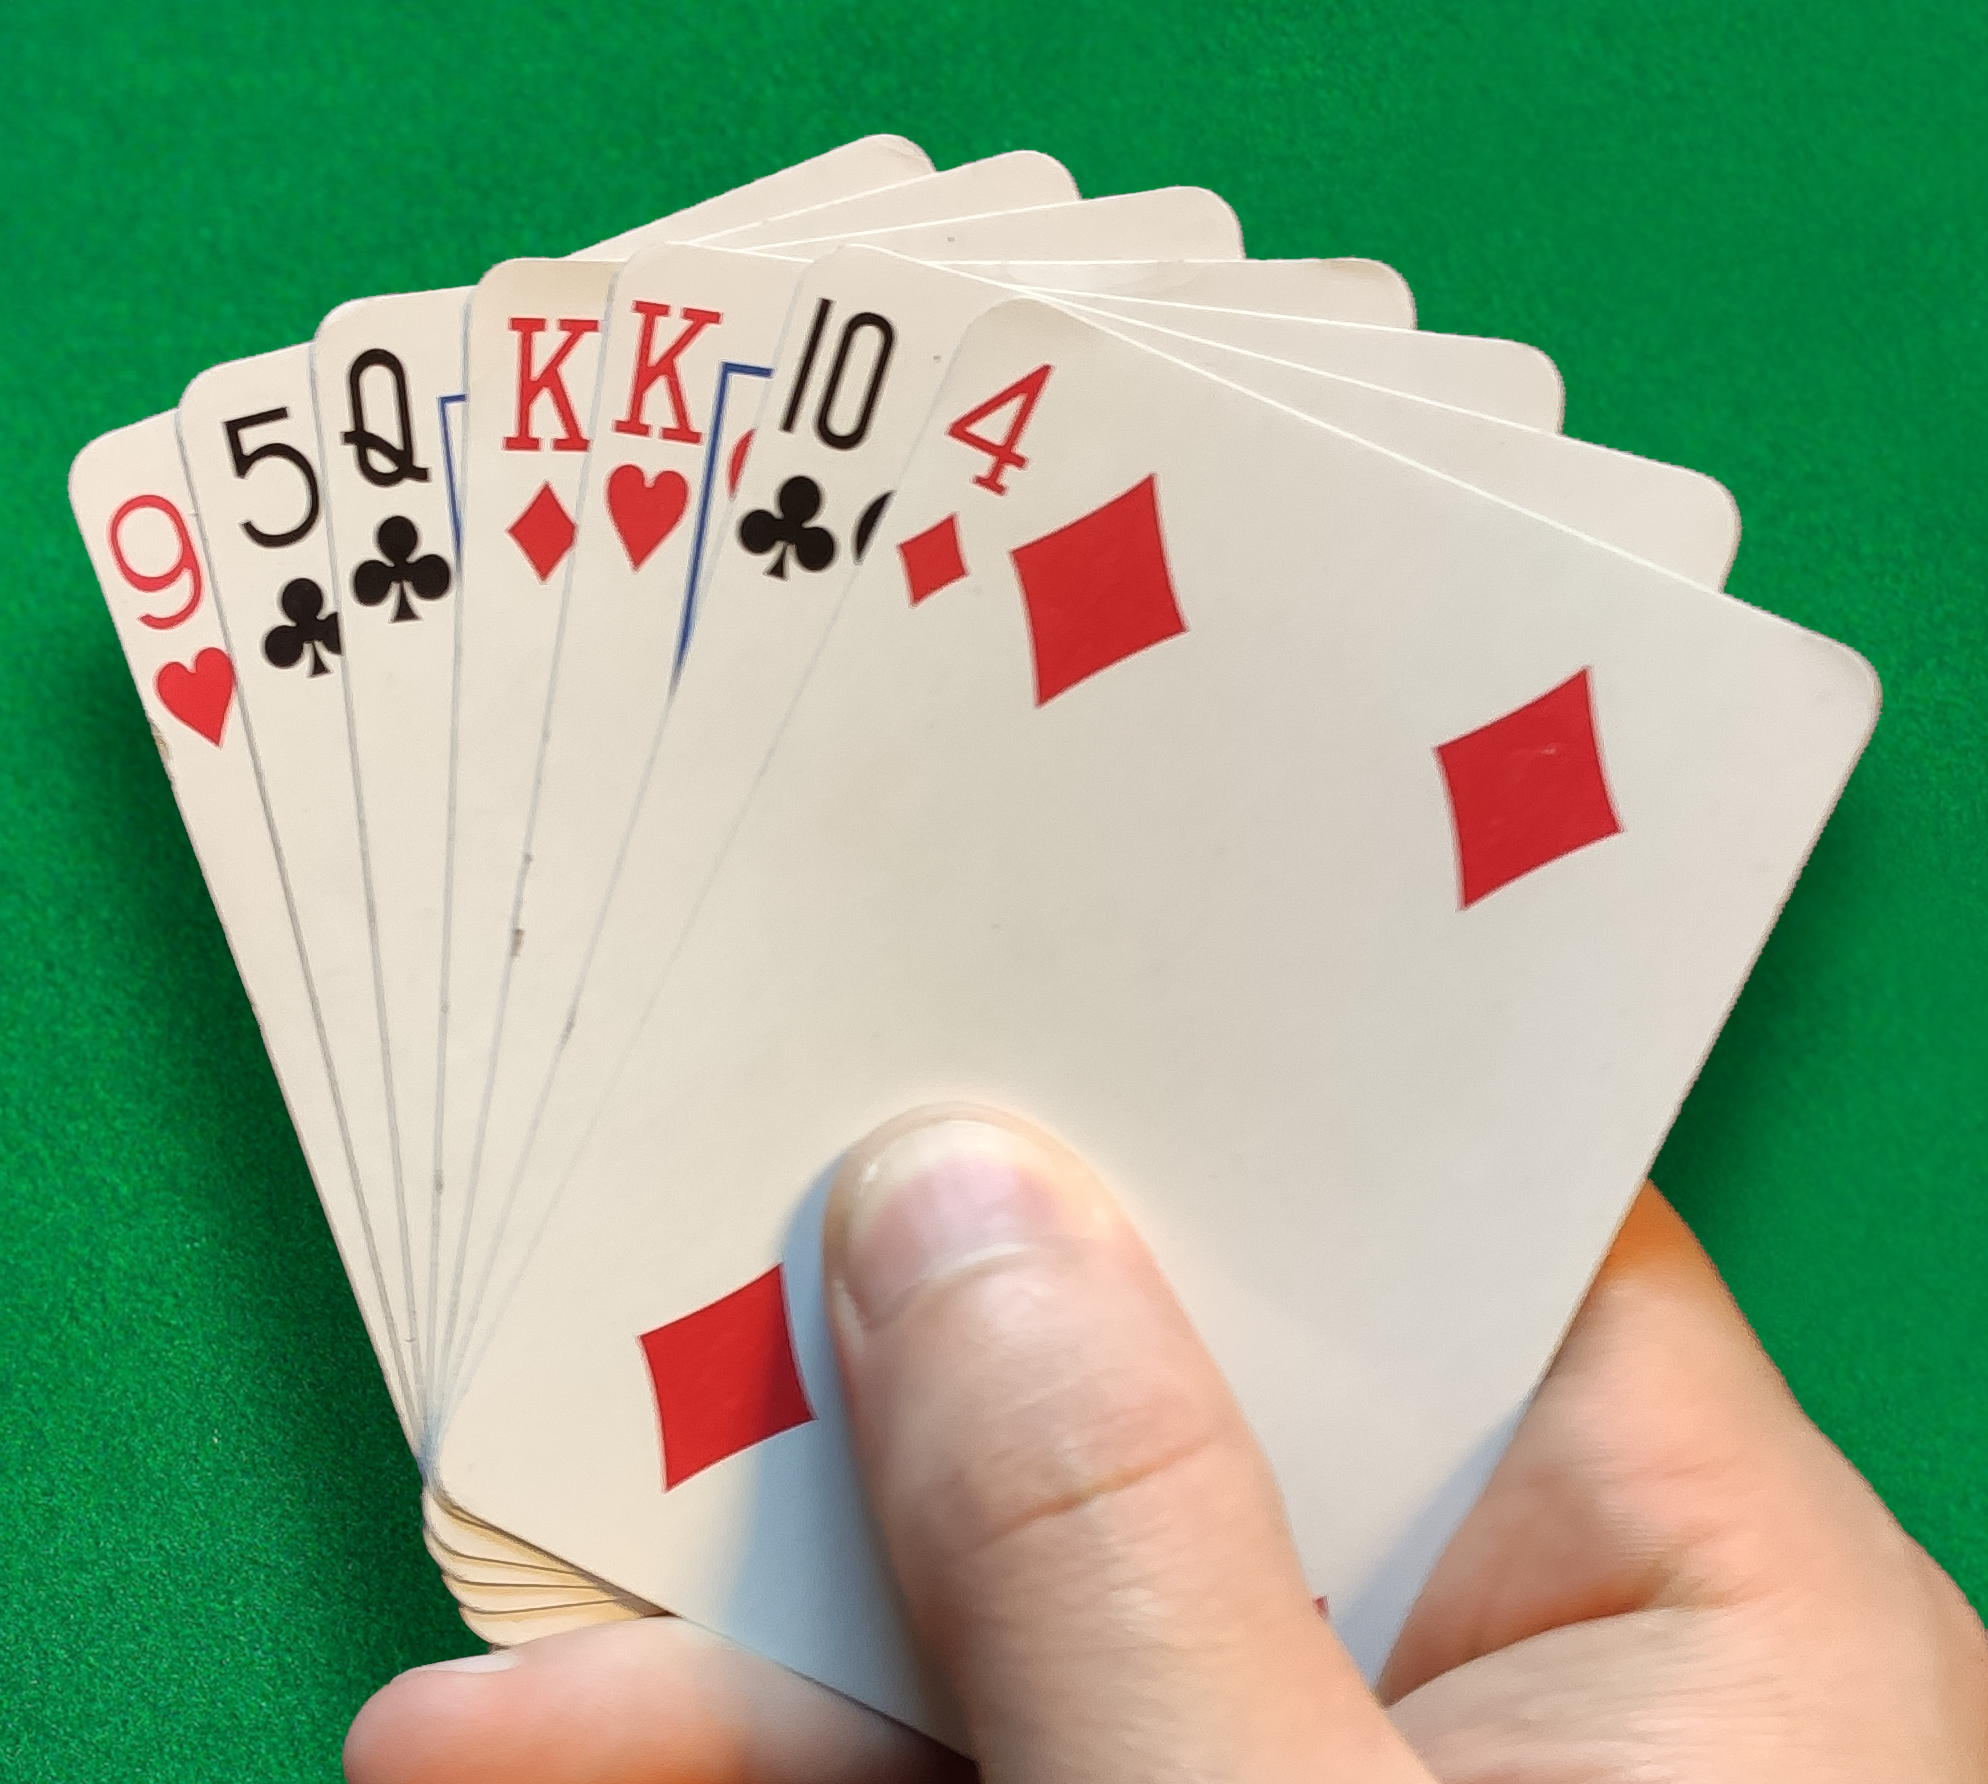
\includegraphics[width=0.33\textwidth]{sample}
	\caption{In Sample 1, Alice has to move at least two cards to sort her hand.}
	  \vspace{-5mm}
\end{wrapfigure}
%\illustration{0.33}{sample.png}{Sample 1: Alice has to move at least two cards to sort her hand.\vspace{-0.5cm}}
The famous card game manufacturer \emph{Greatest Cards Production Company} (GCPC) has just created the brand new card game \emph{\name}.
In this game, everyone gets the same amount of cards -- which might be quite a lot -- and each card belongs to one of four different suits: hearts, diamonds, clubs, or spades.

As huge card game nerds, Alice and her friends are very hyped about meeting up and trying out the card game \mbox{everybody} seems to talk about these days.
Due to a \mbox{traffic} jam, Alice is a bit late to the party and her friends are \mbox{impatiently} waiting for her.
They have already distributed all cards and everybody is ready to go, except for Alice.
She has just picked up her cards and insists on sorting them by suit first.
For that, she repeatedly picks one card from her hand and inserts it somewhere else until her cards are grouped by suit.
Her friends are getting increasingly annoyed with Alice and she wants to sort her cards as quickly as possible.
% Her friends are starting to get annoyed but Alice insists on sorting her cards first.
How many cards does Alice need to move before they can start playing?
%What is the minimal number of cards Alice has to move?

\begin{Input}
    The input consists of:
    \begin{itemize}
        \item One line with a string $s$ ($1\leq|s|\leq 10^5$), representing the suits of Alice's cards as they are initially ordered.
        The string consists of the characters \texttt{h}, \texttt{d}, \texttt{c}, and \texttt{s} (hearts, diamonds, clubs and spades).
    \end{itemize}
\end{Input}

\begin{Output}
    Output a single integer, the minimum number of cards Alice has to move in order to sort the cards by suit.
\end{Output}
